\chapter{Results from the Implementations}~\label{Ch4}

\section{S5 Test with Jijona Parameters}
All the proposals above were presented to the Leadership Team of P\&G Crailsheim to ensure they were aligned with the project scope and the site capability. 

Although Line 15 was not included in the first selection, it was on this Line in which the Jijona Parameters were tested, thus the scrap levels that the line showed were significant during the first days of July 2024. An online meeting was held with one of the line leaders of Jijona to compare the centerline parameters, which correspond to those computed during the process design phase and can be assumed as ideal, with the actual parameters used on the module. 

The different parameters used for producing an S5 pad size are listed in Table~\ref{JJA}, all the values are given in mBar and were taken from~\cite{S5Center}. 

\begin{table}[H]
\centering
\resizebox{\textwidth}{!}{%
\begin{tabular}{ccccccc}
\hline
\textbf{Parameter} & \textbf{JJA   Centerline} & \textbf{JJA Actual} & \textbf{CRA13} & \textbf{CRA15} & \textbf{CRA19} & \textbf{CRA22} \\ \hline
Unit Pressure           & 4000 \pm~2000 & 400  & 3000 & 3500 & 4000 & 5300 \\
Pad Vacuum OS           & 80 \pm~15   & 56   & 154  & 121  & 136  & 91   \\
Pad Vacuum DS           & 80 \pm~15   & 64   & 6    & 125  & 4    & 5    \\
Trim Vacuum OS          & 100 \pm~40  & 128  & 124  & 125  & 4    & -1   \\
Trim Vacuum DS          & 100 \pm~40  & 130  & 6    & 127  & 106  & 99   \\
Transfer Drum   Vacuum  & 30 \pm~50   & 9    & 18   & 24   & 22   & 17   \\
Infeed   Conveyor       & 20 \pm~5   & 22   & 25   & 17   & 19   & 19   \\
Pad Blowoff             & 5000 \pm~1000 & 4000 & 3590 & 4000 & 3970 & 2990 \\
Trim Blowoff            & 6000 \pm~2000 & 4000 & 3590 & 4000 & 3970 & 2990 \\
Trim Chute   Vacuum     & 10 \pm~40   & -    & 9    & 2    & 13   & 14   \\
Transfer Drum   Blowoff & -    & -    & -    & 3000 & -    & -    \\ \hline
\end{tabular}%
}
\caption{STS C\&L S5 Presets Comparison~[Author].}
\label{JJA}
\end{table}

The actual values listed above showed big discrepancies concerning those defined for the centerline, especially those regarding the Pad Vacuum and the Transfer Drum Vacuum, the Team from JJA did not report a specific value for the Trim Chute Vacuum, so it was assumed to be the same as the one in~\cite{S5Center}. As shown in Table~\ref{JJA}, Line 15 is at the moment the only line with a reported Blow-Off Air module installed, then the other lines (including JJA) do not have a preset value for it.

The test was carried out on July 4\textsuperscript{th} 2024 during the morning shift (from 8:37 to 14:20) when the line had achieved a steady state. The chassis changeover was done the day before at 9:00 and the line started running at 1325 ppm until 14:20 when the line speed was changed to 1240 ppm, the Line ran at this speed from 8:37 to 10:50, and then it was decelerated to 1100 ppm for the rest of the Test due to the required PO. Table~\ref{TL15} contains the parameters used during the test, these were obtained using the JJA Centerline values and their uncertainties, and comparing them with the data from the last S5 Run on the Line. 

\begin{table}[H]
\centering
\scriptsize
\begin{tabular}{ccc}
\hline
\textbf{Parameter} & \textbf{CRA15 1240 ppm} &  \textbf{CRA15 1100 ppm} \\
\hline
Unit Pressure                 & 5200      & 5200 \\
Pad Vacuum OS                 & 98        & 72    \\
Pad Vacuum DS                 & 95        & 67     \\ 
Trim Vacuum OS                & 124       & 128     \\
Trim Vacuum DS                & 126       & 131      \\ 
Transfer Drum Vacuum          & 18        & 17        \\
Infeed Conveyor               & 17        & 17         \\
Pad Blowoff                   & 3900      & 3900        \\
Trim Blowoff                  & 3900      & 3900         \\
Trim Chute Vacuum             & 2         & 2             \\
Transfer Drum Blowoff         & 3000      & 3000         \\  \hline
\end{tabular}
\caption{Test Run Parameters~[Author].}
\label{TL15}
\end{table}

Figure~\ref{L15} shows the Line Speed (shown in yellow and with values on the left \textit{y} axis) and the STS Foldback rejections (shown in green and with values on the right\textit{y} axis) from the 3\textsuperscript{rd} to the 5\textsuperscript{th} of July.  A detailed view of the time frame of the test Run is shown in Figure~\ref{L152}. 

During the Test,  there were 6 stops listed most of them related to the Packaging Module, and none of them located on the STS C\&L Module. The JJA team recommended that whenever there was a stop, the Pad and Trim Vacuum Valves should be open completely to allow any clogged fibers or material to leave the system, this practice was followed accordingly during the test, both are butterfly valves. Figure~\ref{valve} shows the above-mentioned valves. 

\begin{figure}[H]
    \centering
    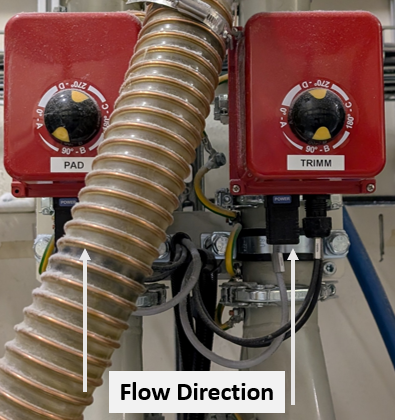
\includegraphics[width=0.4\linewidth]{FIGURES/valves.png}
    \caption{Pad and Trim Vacuum Valves~[Author].}
    \label{valve}
\end{figure}

\begin{figure}[H]
    \centering
    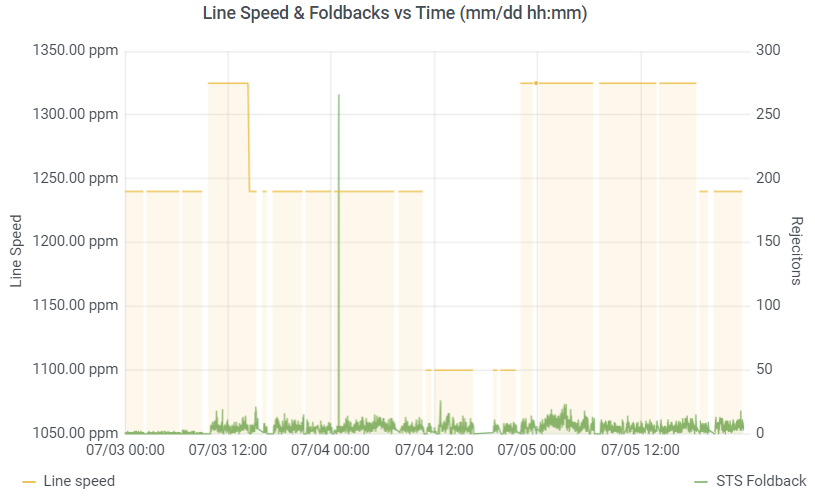
\includegraphics[width=1\linewidth, height = 0.4\textheight]{FIGURES/L15_1.png}
    \caption{Line Speed and STS Foldbacks from the 3\textsuperscript{rd} to the 5\textsuperscript{th} of July~[Author].}
    \label{L15}
\end{figure}

\begin{figure}[H]
    \centering
    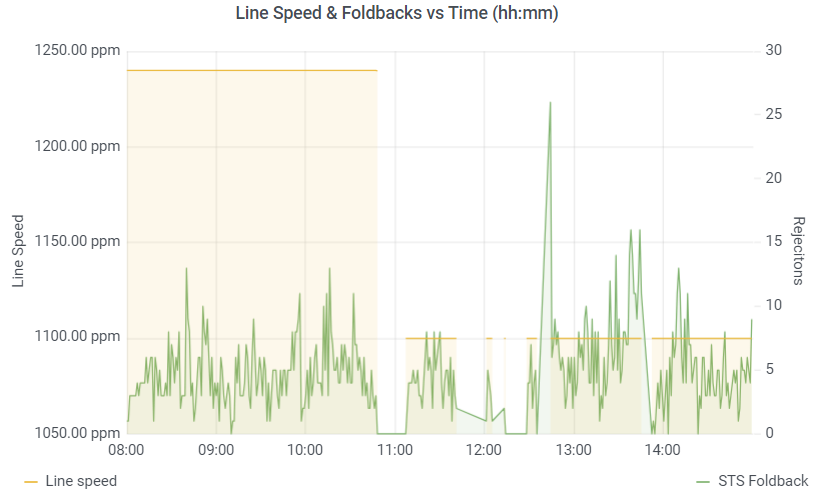
\includegraphics[width=1\linewidth, height = 0.4\textheight]{FIGURES/L15_22.png}
    \caption{Detail View of Test Run Time Frame~[Author].}
    \label{L152}
\end{figure}
%%--------------------------------------------------------------------------%%
\subsection{Findings and Analysis}

The overall performance of the Test was qualified by the Line Team as good, thus the Line did not exhibit unexpected or abnormal behavior, the data in Table~\ref{PR15} relates the performance parameters of the Line and the scrap after the Test in comparison to another S5 Run done on June 20\textsuperscript{th}.

\begin{table}[H]
\centering
\scriptsize
\begin{tabular}{ccc}
\hline
\textbf{Performance Parameter}          & \textbf{CRA15 - 20.06.24} & \textbf{CRA15 - 04.07.24} \\ \hline
PR                             & 75.8\%           & 71.1\%          \\
Total Rejects                  & 8733             & 10135           \\
Total Rejects \%              & 1.75\%           & 2.79\%          \\
Total Scrap                    & 14078            & 11425           \\
Total Scrap \%                & 2.82\%           & 3.15\%          \\
Total STS Foldover Scrap     & 1622             & 1394            \\
Total STS Foldover Scrap \% & 0.32\%           & 0.39\%          \\ \hline
\end{tabular}%
\caption{Line 15 Performance Comparison for S5~[Author].}
\label{PR15}
\end{table}

However, it is worth noticing that the line only ran at 1330 and 1240 ppm on June 20\textsuperscript{th} and not at 1100 ppm. Therefore, analyzing the period during which the Line ran at 1240 ppm on both days, the new performance parameters are given as follows in Table~\ref{PR15-2}.

\begin{table}[H]
\centering
\scriptsize
\begin{tabular}{ccc}
\hline
\textbf{Performance Parameter} & \textbf{CRA15 - 20.06.24 (14:25 - 16:38)} & \textbf{CRA15 - 4.07.24 (8:37 - 10:50)} \\ \hline
PR                           & 96.5\% & 83.4\% \\
Total Rejects                & 1788   & 4899   \\
Total Rejects \%            & 1.11\% & 1.35\% \\
Total Scrap                  & 2037   & 11425  \\
Total Scrap \%              & 1.26\% & 3.15\% \\
Total STS Foldover Scrap     & 1065   & 618    \\
Total STS Foldover Scrap \% & 0.66\% & 0.17\% \\ \hline
\end{tabular}%
\caption{Line 15 Performance Comparison for  S5 at 1240 ppm~[Author].}
\label{PR15-2}
\end{table}

Despite this, Table~\ref{PR15-2} shows that for a Line Speed of 1240 ppm, the STS Foldover scrap is better using the Parameters taken from JJA, showing a total reduction of 74.2\% between the two analyzed dates. Still, this reduction cannot be assumed completely representative, thus the period over which the line ran and produced good product (uptime) at this speed accounts for only 131.4 min, while the uptime of the whole day was 1049.3 min.

The Data shown in Table~\ref{PR15} shows that the test does not enhance the overall PR of the Line, thus the total number of rejects was greater during the test compared to a normal run. Although there were more rejects, the total scrap of the line was lower during the test and there was even less total scrap due to STS Foldover. The STS Foldover was listed as the second-highest reject reason for both cases as shown in Figure~\ref{Scrap2}.

\begin{figure}[H]
    \centering
    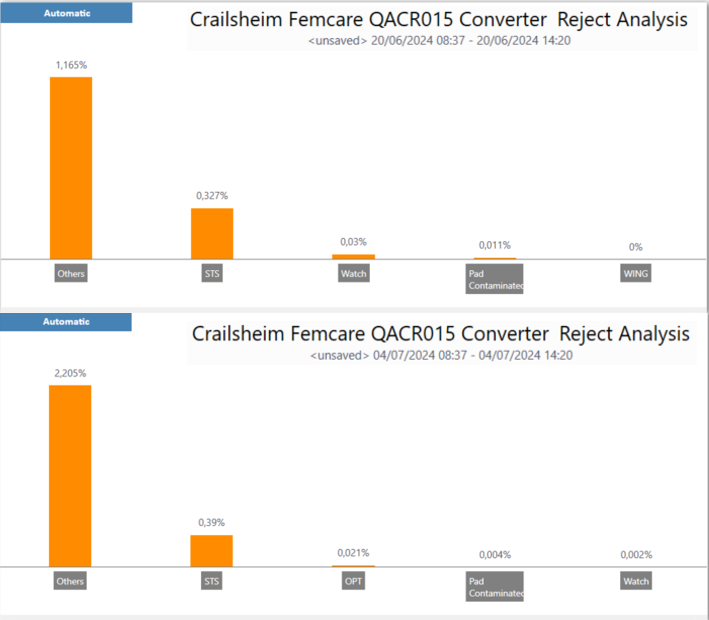
\includegraphics[width = 0.75\linewidth]{FIGURES/scrap2.png}
    \caption{Top 5 Rejects on Line 15 for both case scenarios~[Author].}
    \label{Scrap2}
\end{figure}
\clearpage

On the other hand, the test showed significant changes in the behavior of the Foldbacks. Some images from the Foldbacks before and after changing the parameters were obtained using the Delta Q System from P\&G. Both sets of images show a different nature of foldbacks, on Figure~\ref{AftL15} the rejections exhibit a wrinkle on the lateral edge of the web, whereas Figure~\ref{BefL15} the web is completely folded. A detailed view of the wrinkle and the fold is shown in Figure~\ref{detailL15}.

 \begin{figure}[H]
    \centering
    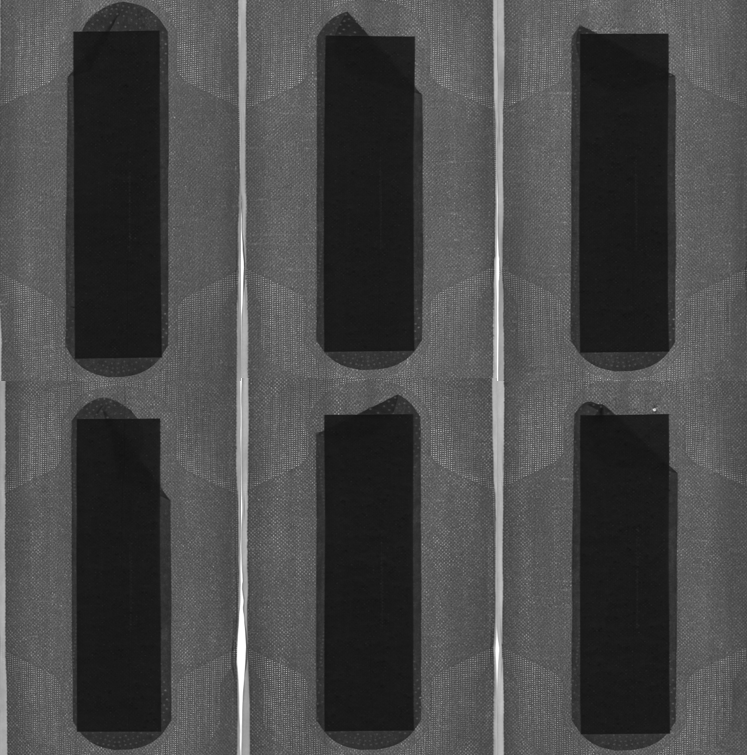
\includegraphics[width=0.5\linewidth]{FIGURES/L15FoldbacksBefore.png}
    \caption{STS Foldovers Before Parameters Set-Up between 6:20 and 7:00~[Author].}
    \label{BefL15}
\end{figure}

\begin{figure}[H]
    \centering
    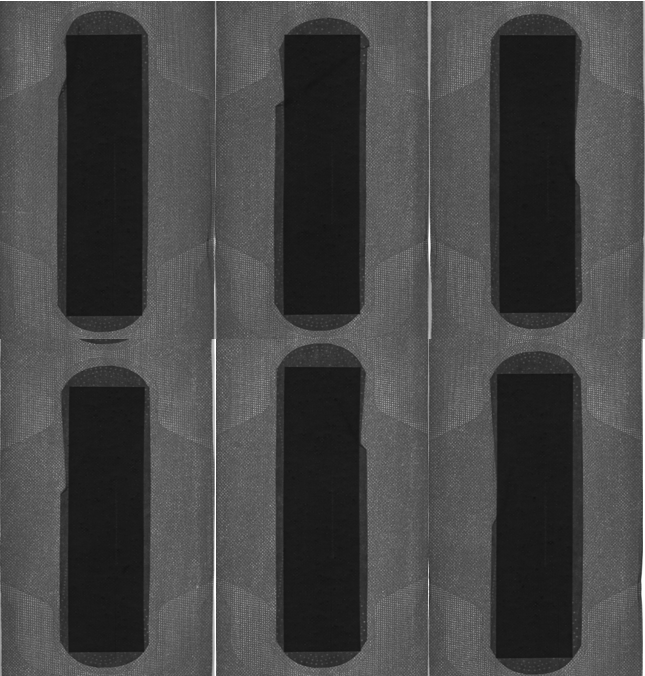
\includegraphics[width=0.5\linewidth]{FIGURES/L15FoldbackAfter.png}
    \caption{STS Foldovers After Parameters Set-Up between 9:00 and 11:30~[Author].}
    \label{AftL15}
\end{figure}

\begin{figure}[H]
\centering
  \begin{subfigure}{0.45\textwidth}
  \centering
    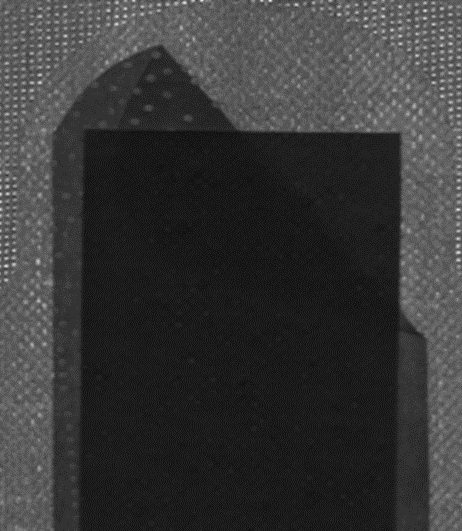
\includegraphics[width=0.8\linewidth]{FIGURES/DetailA_L15.png}
    \caption{Folded STS Detail.}
  \end{subfigure}
  %\hspace{1cm}
  \begin{subfigure}{0.45\textwidth}
  \centering
    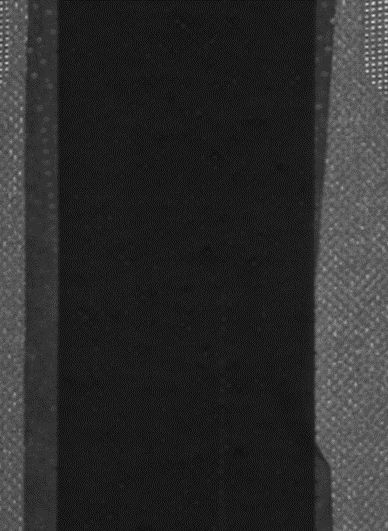
\includegraphics[width=0.8\linewidth]{FIGURES/DetailB_L15.png}
    \caption{Wrinkled Web Detail.}
  \end{subfigure}
  \caption{Detailed View of Rejections Change~[Author].}
    \label{manifolds}
\end{figure}

Figure~\ref{widthL15} shows the STS Web Width against the Foldbacks during the test, fluctuations on the web width for the time frame during which the line ran at 1240 ppm are clear, and the variations imply continuous displacement of the web on the CD direction. According to o~\cite{walker2009taxonomy}, displacement in this direction may lead not only to web wrinkling and buckling but also to uneven cuts of the web. This is noticeable in Figure~\ref{cutL15}, where the uneven cut is labeled as A, and the dark zone labeled as B corresponds to an overlapping Backsheet (the overlapping Backsheet does not influence the STS); it is also noticeable in Figure~\ref{BOEL15} where the Fusion Bond was done unevenly as marked in the ovals A and B.

\begin{figure}[H]
    \centering
    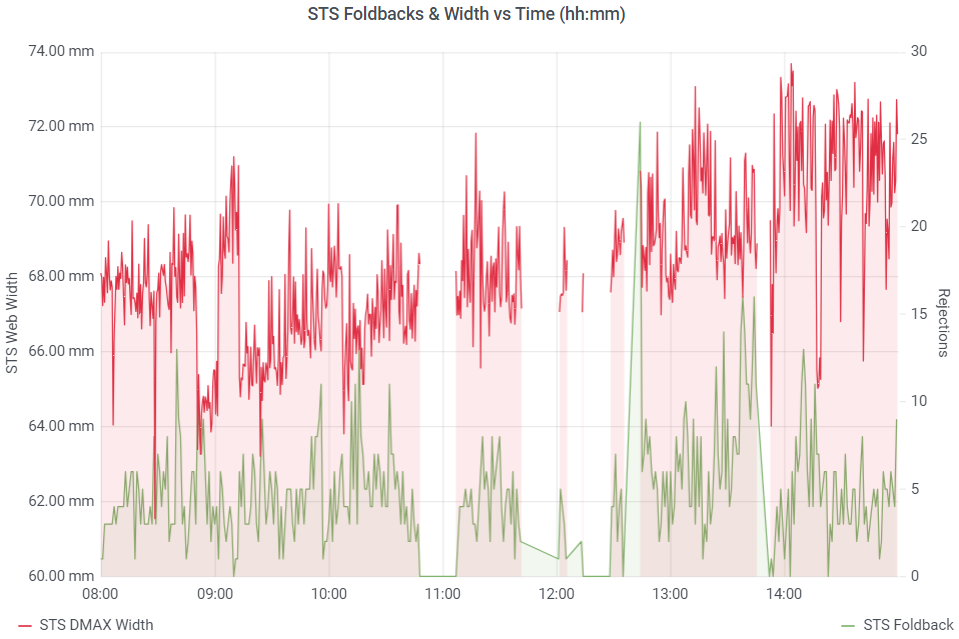
\includegraphics[width=1\linewidth, height=0.4\textheight]{FIGURES/widthL15.png}
    \caption{Web Width and Foldbacks during Test~[Author].}
    \label{widthL15}
\end{figure}

\begin{figure}[H]
    \centering
    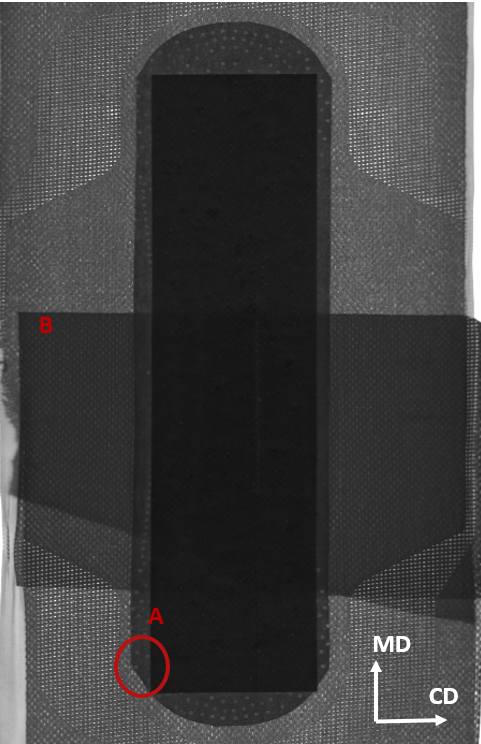
\includegraphics[width=0.5\linewidth]{FIGURES/CutL15.png}
    \caption{Uneven Cut due to Web Displacement in CD Direction~[Author].}
    \label{cutL15}
\end{figure}

\begin{figure}[H]
    \centering
    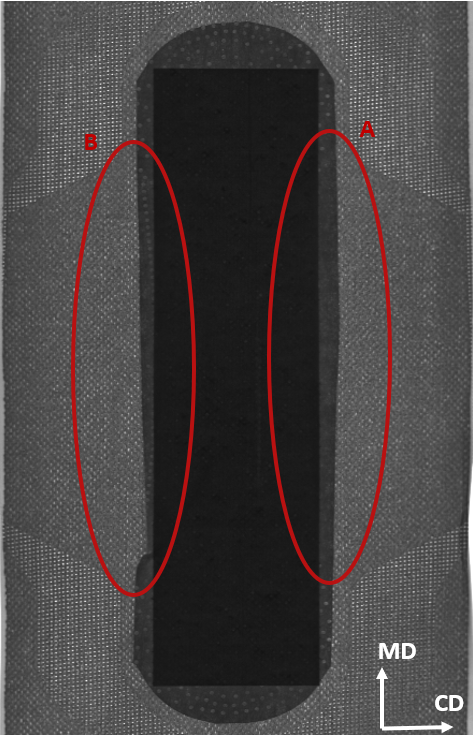
\includegraphics[width=0.5\linewidth]{FIGURES/BOEL15.png}
    \caption{Uneven Bonding due to Web Displacement in CD Direction~[Author].}
    \label{BOEL15}
\end{figure}

%%-------------------------------------------------------%%
\section{S1 and S3 Test with the new Vacuum Manifold}

The manifolds are designed to secure the STS web after it has been cut to the required shape, utilizing the pad vacuum mechanism. Additionally, they hold the residual web pieces post-cutting via the trim vacuum function, using the pad blow-off mechanism they facilitate the transference of the shaped web to the Transfer Drum by blowing air. Simultaneously, the trim blow-off mechanism directs the remaining web pieces into the chute vacuum. These operations are enabled by the distinct air chambers integrated within the manifold structure.

Figures~\ref{CRAMan1} to~\ref{BUDMan2} show the current manifold installed on the S1 and S3 units on CRA and BUD, respectively.

\begin{figure}[H]
    \centering
    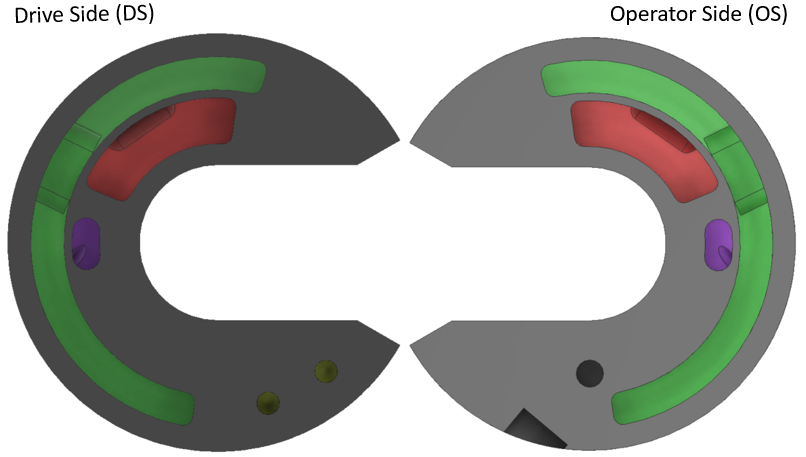
\includegraphics[width=1\linewidth]{FIGURES/S1CRAMan.png}
    \caption{S1 Vacuum Manifold used in CRA~[Author].}
    \label{CRAMan1}
\end{figure}

\begin{figure}[H]
    \centering
    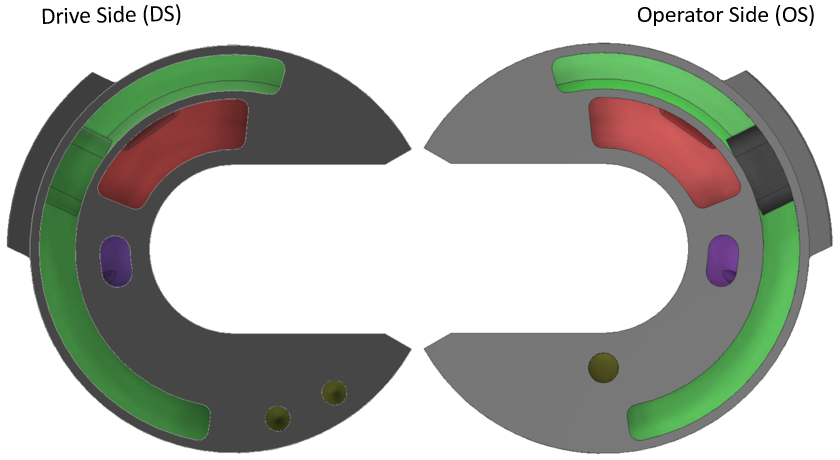
\includegraphics[width=1\linewidth]{FIGURES/S3CRAMan.png}
    \caption{S3 Vacuum Manifold used in CRA~[Author].}
    \label{CRAMan2}
\end{figure}

\begin{figure}[H]
    \centering
    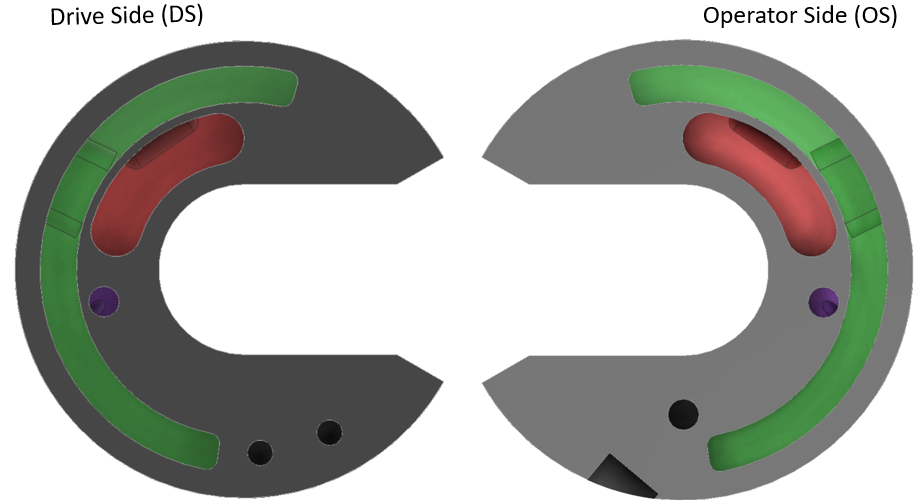
\includegraphics[width=1\linewidth]{FIGURES/S1BUDMan.png}
    \caption{S1 Vacuum Manifold used in BUD~[Author].}
    \label{BUDMan1}
\end{figure}

\begin{figure}[H]
    \centering
    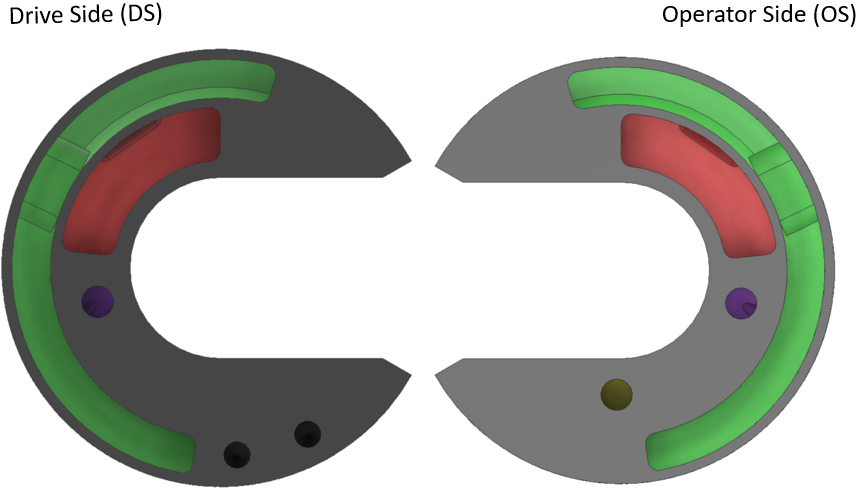
\includegraphics[width=1\linewidth]{FIGURES/S3BUDMan.png}
    \caption{S3 Vacuum Manifold used in BUD~[Author].}
    \label{BUDMan2}
\end{figure}
\clearpage

The actual manifolds used in CRA differ from the ones used in BUD in mainly the following aspects:

\textbf{Pad Vacuum Chamber:} The chamber is marked with red in Figures~\ref{CRAMan1} to~\ref{BUDMan2}. Though the geometry of the chamber looks more or less the same for the S1 manifold from BUD and CRA, as well as for the S3 manifold from CRA, there is a clear change in the geometry of the chamber for the S3-BUD Manifold. The volumetric capacity of each chamber is summarized in Table~\ref{PadVacuumVol}:
    \begin{table}[H]
    \centering
    \scriptsize
    \begin{tabular}{cc}
    \hline
    \textbf{Manifold - Location} & \textbf{Volumetric Capacity cm$^3$} \\ \hline
    S1 - CRA                     & 27.22                              \\
    S1 - BUD                     & 29.12                              \\
    S3 - CRA                     & 26.10                              \\
    S3 - BUD                     & 29.49                              \\ \hline
    \end{tabular}%
    \caption{Pad Vacuum Chamber Volume Capacity~[Author].}
    \label{PadVacuumVol}
    \end{table}
    
The difference in the capacity between the manifolds from both sites is not only a geometric feature from the designs but have also implications process-wise, then this chamber is responsible for holding the STS web once it is cut in the Pad shape. This means, that the manifold from BUD holds the web tighter and helps to keep it in place for more time than the current manifolds from CRA.

Moreover, the position of the chamber from both manifolds differs, while for the BUD ones the chamber begins exactly at 90$^{\circ}$, and for the CRA ones it begins at 82$^{\circ}$ and 84$^{\circ}$ for S1 and S3 sizes respectively~\cite{manifold, manifold2}. This slight angle change implies holding the web early in the module. 

\textbf{Pad Blow-Off Chamber:} The chamber is marked with purple in Figures~\ref{CRAMan1} to~\ref{BUDMan2}. There is a clear change in the geometry from both chambers as well as in the position of it. Table~\ref{PadVacuumVol2} shows the difference in volumetric capacity due to this geometry change from the manifolds.
    \begin{table}[H]
    \centering
    \scriptsize
    \begin{tabular}{cc}
    \hline
    \textbf{Manifold - Location} & \textbf{Volumetric Capacity cm$^3$} \\ \hline
    S1 - CRA                     & 4.34                              \\
    S1 - BUD                     & 2.03                              \\
    S3 - CRA                     & 3.89                              \\
    S3 - BUD                     & 2.03                              \\ \hline
    \end{tabular}%
    \caption{Pad Blow-Off Chamber Volume Capacity~[Author].}
    \label{PadVacuumVol2}
    \end{table}

The CRA manifolds show a greater volumetric capacity, therefore they can blow more air, leading to a faster web transference to the Transfer Drum. Nevertheless, the chamber is symmetric to the middle line of the manifold, whereas the BUD manifolds have this chamber located at 13.3$^{\circ}$ from the middle line (clockwise), see Figure~\ref{ManLoc}.

\begin{figure}[H]
\centering
  \begin{subfigure}{0.4\textwidth}
  \centering
    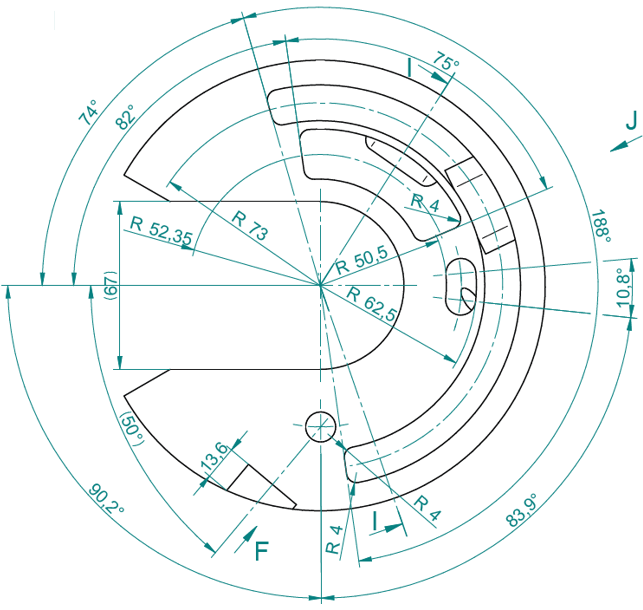
\includegraphics[width=1\linewidth]{FIGURES/CRAloc.png}
    \caption{CRA S3 Manifold.}
  \end{subfigure}
  %\hspace{1cm}
  \begin{subfigure}{0.4\textwidth}
  \centering
    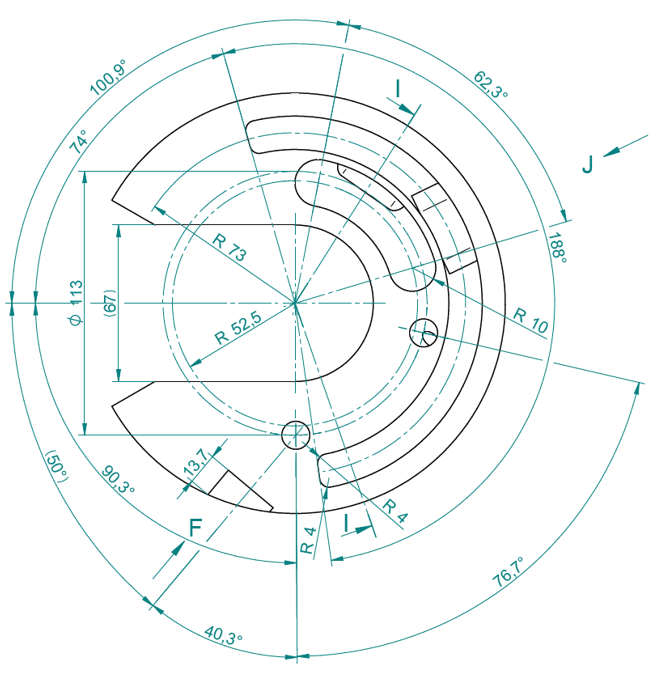
\includegraphics[width=1\linewidth]{FIGURES/BUDloc.png}
    \caption{BUD S3 Manifold.}
  \end{subfigure}
  \caption{Blow-Off Chambers Location~\cite{manifold2}.}
    \label{ManLoc}
\end{figure}

This design feature from CRA aims to start the blow-off earlier to have a better process handover, but this also represents a bigger chance of having false air, i.e., air that is supposed to act on the web, but that is being dispersed and not entering the air channel of the knife roll. This case is also known as \textit{falsche Luft}. Figure~\ref{channel} shows the different air channels of the knife roll of the STS C\&L Unit.
\begin{figure}[H]
    \centering
    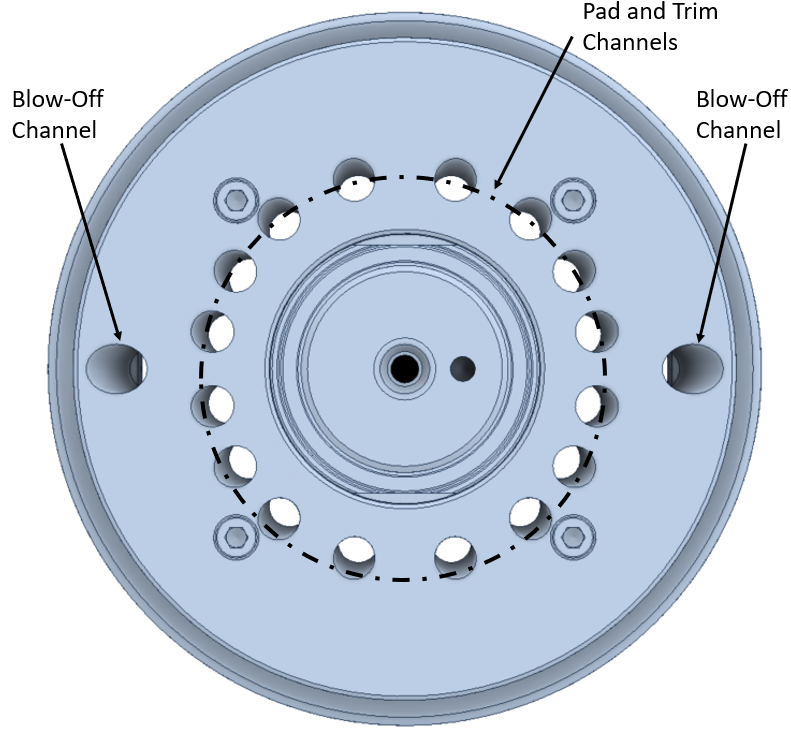
\includegraphics[width=0.7\linewidth]{FIGURES/Channel.png}
    \caption{Vacuum Channels~[author].}
    \label{channel}
\end{figure}

The BUD Manifolds were tested on Lines 16 for S3 (from August 16\textsuperscript{th} to 20\textsuperscript{th}), and on Line 19 for S1 (from August 1\textsuperscript{st} to 9\textsuperscript{th}). 

%%--------------------------------------------------------------------------%%
\subsection{Findings and Analysis}
The changeover for Line 19 was done on August 1\textsuperscript{st} at 7:30 after the Line had stabilized. During the replacement of the manifolds on Line 19, the CRA manifolds showed surface wear generated by the friction between the knife roll and the inner part of the manifold. It also exhibited ink contamination, and clogged fibers inside the vacuum chambers. The clogging of the Fibers was noticeable in the pipe fittings of the manifold and at the inlet of the manifold as well. See Figures~\ref{CRAMan3}, ~\ref{fibers1}, and~\ref{fibers2}.

This situation was not the same for Line 16, thus the manifolds were installed in the unit without any previous run as a request from the Line Leader. Then, the unit was completely prepared on the Workshop.
\begin{figure}[H]
    \centering
    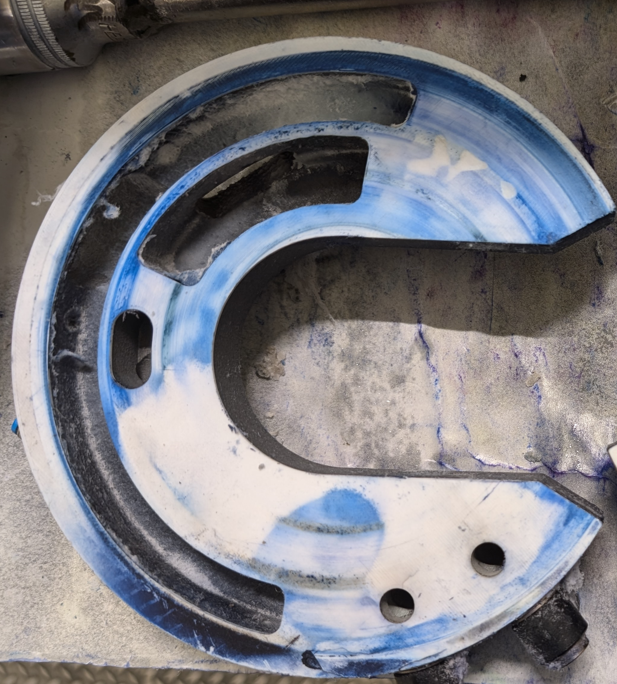
\includegraphics[width=0.4\linewidth]{FIGURES/CRAMan3.png}
    \caption{CRA S1 DS Manifold from Line 19~[Author].}
    \label{CRAMan3}
\end{figure}

\begin{figure}[H]
\centering
  \begin{subfigure}{0.45\textwidth}
  \centering
    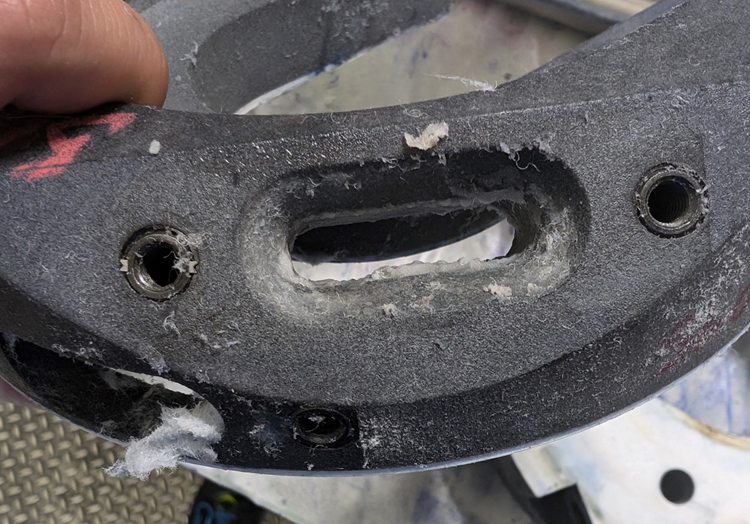
\includegraphics[width=1\linewidth]{FIGURES/Fib1.png}
    \caption{Inlets.}
  \end{subfigure}
  %\hspace{1cm}
  \begin{subfigure}{0.45\textwidth}
  \centering
    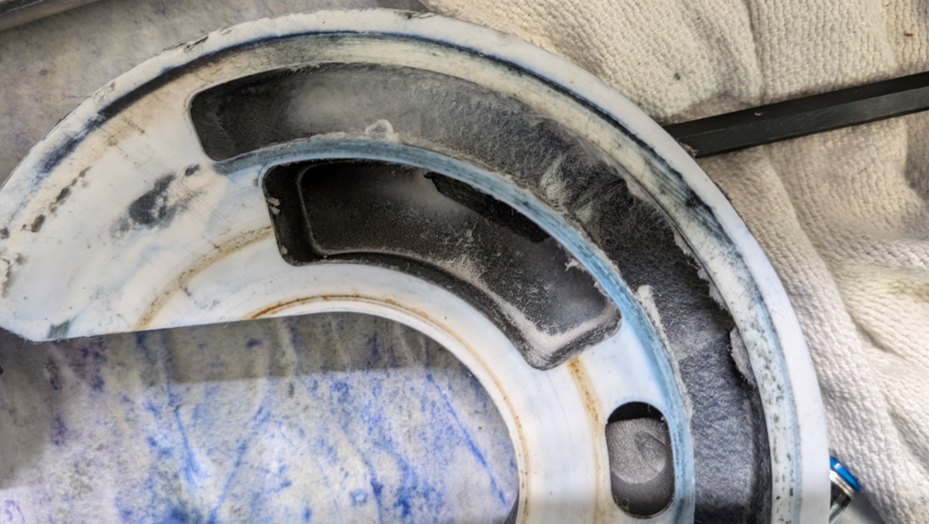
\includegraphics[width=1.1\linewidth]{FIGURES/Fib2.png}
    \caption{Chambers.}
  \end{subfigure}
  \caption{Clogged Fibers in CRA Manifold Inlets and Chambers~[Author].}
    \label{fibers1}
\end{figure}


\begin{figure}[H]
\centering
  \begin{subfigure}{0.45\textwidth}
  \centering
    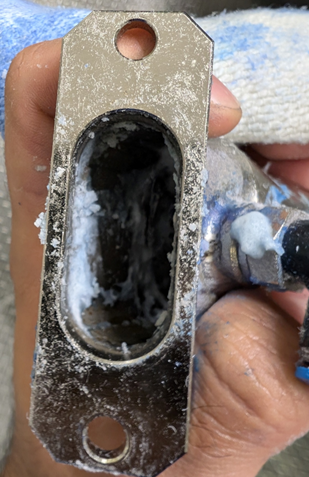
\includegraphics[width=0.8\linewidth]{FIGURES/Fib3.png}
    \caption{Pipe Fitting OS.}
  \end{subfigure}
  %\hspace{1cm}
  \begin{subfigure}{0.45\textwidth}
  \centering
    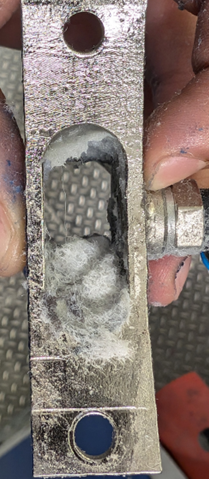
\includegraphics[width=0.7\linewidth]{FIGURES/Fib4.png}
    \caption{Pipe Fitting DS.}
  \end{subfigure}
  \caption{Clogged Fibers in CRA Manifold Fittings~[Author].}
    \label{fibers2}
\end{figure}

Figures~\ref{L19_Test} and~\ref{L16_Test} show the line speed against the foldbacks during the test run. on their respective dates.
\begin{figure}[H]
    \centering
    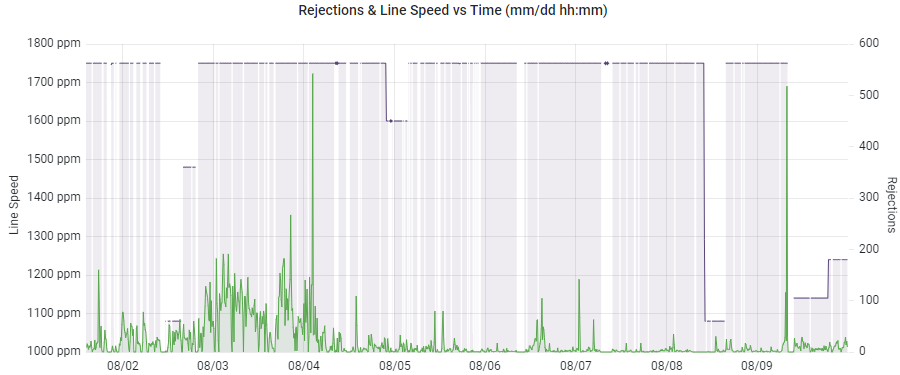
\includegraphics[width=1\linewidth]{FIGURES/L19_Test.png}
    \caption{Line Speed and Foldbacks against Time during Test in Line 19~[Author].}
    \label{L19_Test}
\end{figure}

\begin{figure}[H]
    \centering
    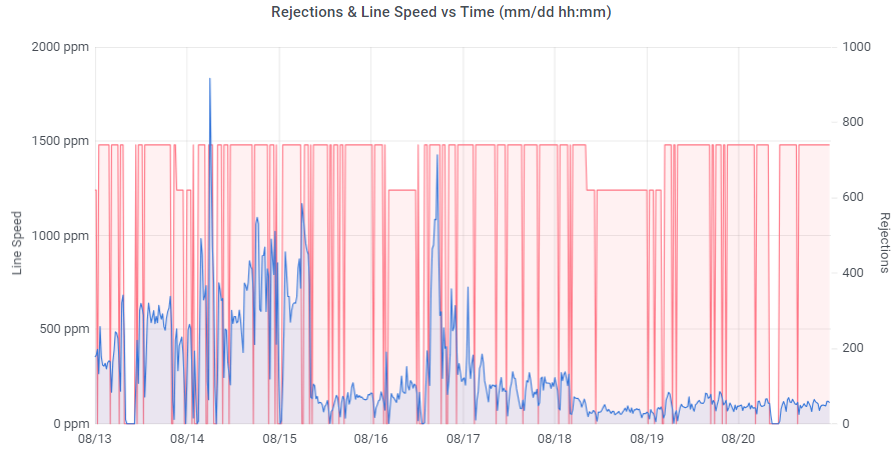
\includegraphics[width=1\linewidth]{FIGURES/L16_Test.png}
    \caption{Line Speed and Foldbacks against Time during Test in Line 16~[Author].}
    \label{L16_Test}
\end{figure}

The overall performance of the both Test was qualified by the Line Team as good thus the Line did not exhibit unexpected or abnormal behavior, the data in Table~\ref{PR15} relates the performance parameters of the Line and the scrap after the Test in comparison to another S5 Run done on June 20\textsuperscript{th}.

\begin{table}[H]
\centering
\scriptsize
\begin{tabular}{ccc}
\hline
\textbf{Performance Parameter}          & \textbf{CRA15 - 20.06.24} & \textbf{CRA15 - 04.07.24} \\ \hline
PR                             & 75.8\%           & 71.1\%          \\
Total Rejects                  & 8733             & 10135           \\
Total Rejects \%              & 1.75\%           & 2.79\%          \\
Total Scrap                    & 14078            & 11425           \\
Total Scrap \%                & 2.82\%           & 3.15\%          \\
Total STS Foldover Scrap     & 1622             & 1394            \\
Total STS Foldover Scrap \% & 0.32\%           & 0.39\%          \\ \hline
\end{tabular}%
\caption{Line 15 Performance Comparison for S5~[Author].}
\label{PR15}
\end{table}